\def\year{2018}\relax
%File: formatting-instruction.tex
\documentclass[letterpaper]{article} %DO NOT CHANGE THIS
\usepackage{aaai18}  %Required
\usepackage{times}  %Required
\usepackage{helvet}  %Required
\usepackage{courier}  %Required
\usepackage{url}  %Required
\usepackage{graphicx}  %Required
\frenchspacing  %Required
\usepackage{amsmath}
\usepackage{amsthm}
\usepackage{graphicx}
\usepackage{subfig}
\usepackage{amssymb}
\setlength{\pdfpagewidth}{8.5in}  %Required
\setlength{\pdfpageheight}{11in}  %Required
\newtheorem{theorem}{Theorem}
\newtheorem*{remark}{Remark}
%PDF Info Is Required:
  \pdfinfo{
/Title (Complex Unitary Recurrent Neural Networks using Scaled Cayley Transform)
/Author (Author)}
\setcounter{secnumdepth}{2}  
 \begin{document}
% The file aaai.sty is the style file for AAAI Press 
% proceedings, working notes, and technical reports.
%
\title{Complex Unitary Recurrent Neural Networks using Scaled Cayley Transform}
\author{Authors }
\maketitle
\begin{abstract}
Recurrent neural networks (RNNs) have been successfully used in wide range of sequential problems. Despite this success, RNNs suffer from the \textit{vanishing or exploding gradients} problem. One recent method “scaled Cayley orthogonal recurrent neural network” (scoRNN) addresses this issue by maintaining an orthogonal recurrent weight matrix by parametrizing a skew-symmetric matrix through a scaled Cayley transform. The initial implementation of scoRNN used an orthogonal recurrent matrix, yet complex unitary recurrent representation could have been used. We extend the idea of scoRNN architecture and use unitary recurrent weight matrix by parameterizing a skew-hermition matrix through a scaled Cayley transform. We discuss the advantage and the competitive performance of our complex RNN has over the traditional scoRNN and implementation issues. In several experiments, the extended method scaled cayley unitary recurrent neural network ( scuRNN) achieves comparable results with other unitary recurrent neural networks. 
\end{abstract}

\section{Introduction}
\noindent Recurrent neural networks (RNNs) have been shown to have an outstanding performance in a wide range of problems, including image recognition \cite{Krizh12}, speech recognition \cite{Hinton12} and natural language processing \cite{Collobert11}. A main difficulty when training using the gradient descent approach is the \textit{vanishing or exploding gradients} problem \cite{Hochreiter91}. The exploding gradient problem refers to the large increase in the norm of the gradient during training caused by to the explosion of the long term components, which can grow exponentially more than short term ones. The vanishing gradients problem is the opposite phenomena of exploding gradients and can be thought as large decrease in the norm of the gradient during training. Vanishing gradients makes it difficult to know which direction the parameter should move to minimize the loss function. On the other hand exploding gradients can make leaning unstable.\\ 

\noindent Currently, many architectures are available to address this issue. For example, Long Short-Term Memory network (LSTMs) \cite{Hochreiter97} and Gated Recurrent Unit recurrent neural network (GRU) \cite{Cho14}  use gating mechanisms to control when information is retained  or  discarded. Some recent popular methods address this issue by maintaining an unitary recurrent weight matrix. Such methods are first used by \cite{Arjo16} and then by \cite{Wisdom16}. We follow the convention of \cite{Wisdom16} and call Full-capacity uRNN for the network used in \cite{Wisdom16} and call restricted-capacity uRNN for the network used in \cite{Arjo16}. More recently, the  scoRNN architecture  used orthogonal recurrent weight matrix instead of unitary matrix \cite{kyle17}. This scoRNN parametrization keeps exact orthogonality up to floating point precision,verses restricted-capacity and full capacity uRNNs.\\ 

\noindent In this paper, we address the main drawback of the scoRNN paper by making the recurrent weight matrix to be unitary and then make the scaling matrix to be unitary diagonal and allow to be learnable from the gradient decent approach, instead of the diagonal matrix being $\pm 1,$ and using the number of negative ones in the diagonal to be hyper parameter. In other words, we consider RNNs with a recurrent matrix taken from the set of all unitary matrices, which can be parameterized using the scaled Cayley transform of a skew-hermitian matrix. Extended update scheme will be provided for the complex valued case, using Writinger Calculus \cite{Kreutzdelgado09}. This complex RNN overcome the difficulty of tuning the number of negative ones in the scaling diagonal matrix for the each particular task. To overcome this difficulty we use scaled diagonal matrix initialized to be random unitary diagonal matrix and allow it to be trainable using simple gradient decent based update scheme. The experiments done by this architecture provides that the better or comparable results can be achieved without spending time to tune the hyper parameter given in scoRNN paper.

\noindent In the next section,  we discuss the background and motivation of the current RNN structure. In section 3 we discuss our proposed model with the update scheme for both the recurrent matrix, and scaled diagonal unitary matrix with some introduction to the Writinger calculus. In section 5 we include experiments that illustrate comparable results.

\section{Background}
\subsection{Recurrent Neural Networks}
\noindent A single hidden layer recurrent neural network (RNN) is a dynamical system uses an input sequence $x = (x_1, x_2, ... , x_{\tau})$ where $x_i \in \mathbb{R}^m$, to produce an output sequence $y = (y_1, y_2, ... , y_{\tau})$ where each $y_i \in \mathbb{R}^p$ is given recursively by the following: 
\begin{align*}
\textbf{h}_t & = \sigma \left(Ux_t + W h_{t-1} + b\right) \\
y_t & = Vh_t + c
\end{align*}

\noindent The parameters of this RNN are as follows:  $U \in \mathbb{R}^{n \times m}$, input-hidden transform parameters; $W \in \mathbb{R}^{n \times n}$, hidden recurrent matrix; $b \in \mathbb{R}^n$, recurrent bias; $V \in \mathbb{R}^{p \times n}$, hidden-output transform parameters; $c \in \mathbb{R}^p$, output bias.  Here $m$ is the data input size, $n$ is the number of hidden units, and $p$ is the output data size. $h = (h_0, \ldots, h_{\tau})$, $h_i \in \mathbb{R}^n$ is the hidden layer state at time $i$ and $\sigma(\cdot)$ is the activation function, which is often a pointless nonlinearity such as a hyperbolic tangent function or rectified linear unit \cite{Nair10}.\\

%\subsection{Vanishing and exploding gradients}
\noindent Recurrent Neural Networks (RNNs) are designed to process sequential data, but suffer from \textit{vanishing or exploding gradients}. For a typical classification problem, the RNN is designed to only output a vector at the end of the sequence $t = \tau$.  In this case, we must backpropagate through the loss function at time $\tau$.  Looking at the $\frac{\partial L}{\partial h_t}$ term, we have,

\[
	\frac{\partial L}{\partial h_t} = \frac{\partial L}{\partial h_{\tau}}\frac{\partial h_{\tau}}{\partial h_{\tau-1}}...\frac{\partial h_{t+1}}{\partial h_{t}} = \frac{\partial L}{\partial h_{\tau}}D_{\tau}WD_{\tau-1}W ... D_{t+1}W.  
\]
where $D_t = \text{diag}\left(\sigma'\left(z_t \right)\right)$ is a diagonal matrix with diagonal entries of the form $\sigma'\left(z_t\right)_i$.

\noindent Taking the matrix 2-norm on both sides we obtain the following inequality,
\begin{gather}
\label{norminequility}
\left\lVert \frac{\partial L}{\partial h_t}\right\rVert_2 \leq \left\lVert \frac{\partial L}{\partial h_{\tau}} \right\rVert_2 \left\lVert D_{\tau} \right\rVert_2 \left\lVert D_{\tau-1} \right\rVert_2 ... \left\lVert D_{t+1} \right\rVert_2 \left\lVert W \right\rVert^{\tau - t}_2.
\end{gather}
\noindent Now, if $\left\lVert W \right\rVert_2 < 1$, we see from the above inequality (\ref{norminequility}) that the upper bound of the inequality goes to zero as $\tau - t$ goes to infinity.  This phenomenon is known as the vanishing gradient problem.  In this case, the derivative will go to zero and so gradient descent will not cause the current weights to update which in turn causes no change in the loss function.  As a result, any long-term dependencies will be lost.\\
\noindent If $\left\lVert W \right\rVert_2 > 1$, the right hand side of the inequality will become unbounded as $\tau - t$ goes to infinity. This is known as the exploding gradient problem.  In this case, gradient descent will result in too large of an update step to occur which may cause the model to oscillate around or overstep a local minimum.\\

\noindent Now, if $W$ is unitary or orthogonal, then $\left\lVert W \right\rVert_2 = 1$ and the inequality \ref{norminequility} becomes

\begin{gather}
\label{norminequility2}
\left\lVert \frac{\partial L}{\partial h_t}\right\rVert_2 \leq \left\lVert \frac{\partial L}{\partial h_{\tau}} \right\rVert_2 \left\lVert D_{\tau} \right\rVert_2 \left\lVert D_{\tau-1} \right\rVert_2 ... \left\lVert D_{t+1} \right\rVert_2 .
\end{gather}
\noindent With the right selection of the nonlinear function, the right hand side of the inequality \ref{norminequility2} should not vanish or become unbounded.\\

\subsection{Unitary RNNs and scoRNN}
The uRNN follows the structure given in recurrent neural network section, and main difference comes with the way it parameterize the recurrent weight matrix. The restricted capacity uRNN proposed by \cite{Arjo16} introduce a parametrization of the recurrent matrix $W$ using product consisting of diagonal matrices of norm 1, complex householder reflection matrices,discrete Fourier transformation matrices. The Efficient Unitary RNN (EURNN) by \cite{jing16} and orthogonal RNN (oRNN) by \cite{Mhammadi17} parametrize in a similar manner with produnct of Givens rotation matrices and Householder reflection matrices, respectively. The full capacity uRNN proposed by \cite{Wisdom16} construct s unitary matrix recursively from the previous time step by moving along a curve on the Stiefel manifold 
$$\{W \in \mathbb{C}^{n \times n} | W^*W =I\}.$$ 
The scoRNN architecture by \cite{kyle17}, the orthogonal recurrent matrix $W$ is formed by the scaled Cayley transform:
$$W = (I+A)^{-1}(I-A)D. $$
In the training process scoRNN uses a fixed Diagonal matrix $D$ containing -1s and +1s in the diagonal and update the skew-symmetric matrix using gradient decent optimization:
$$A ^{(k+1)} = A^{(k)} -\lambda \frac{ \partial L(W(A^{(k)})}{\partial A} ,$$
and then use scaled Cayley transform to update the recurrent matrix:
$$ W^{(k+1)} = (I+A ^{(k+1)})^{-1}(I-A ^{(k+1)})D.  $$

\section{Scaled Cayley Unitary RNN}

\noindent The architecture for the current method uses the uRNN structure presented in \cite{Arjo16} which contains the following system with real inputs $\textbf{x}_t \in \mathbb{R}^m$, complex valued hidden states $\textbf{h}_t\in \mathbb{C}^n$, and real valued outputs $\textbf{y}_t \in \mathbb{R}^l:$ 
\begin{align*}
 \textbf{h}_t &= \sigma_{\textbf{b}}(\overbrace{W\textbf{h}_{t-1} +U\textbf{x}_t}^{\textbf{z}}) \\
 \textbf{y}_t &= V \textbf{h}_t +c,
\end{align*}

where $\sigma_{\textbf{b}}(\cdot)$ is the activation function; $W \in \mathbb{C}^{n \times n}$, unitary hidden-hidden recurrent matrix; $U \in \mathbb{C}^{n\times m}$, input-hidden matrix; $\textbf{b}\in \mathbb{R}^n$ nonlinearity bias parameters; $V \in \mathbb{C}^{l\times n}$, hidden-output transformation matrix; and $\textbf{c} \in \mathbb{R}^l,$ output bias.\\

\noindent We parametrized $W$ using the Cayley transform of a skew-Hermitian matrix $A$, scaled by an appropriate unitary diagonal matrix $D$, so that the parameterization guarantee that the modulus of the elements in $A$ less than one. This parametrization gives access to every unitary matrices in the training process thanks to the following result from \cite{kahan06} as detailed in the paper \cite{kyle17}.\\

\begin{theorem}
Every unitary matrix $W$ can be expressed as 
$$ W = (I+A)^{-1}(I+A)D$$ where $A =[a_{ij}]$ is skew-Hermitian with $|a_{ij}| \leq 1$ and $D$ is a unitary diagonal matrix.
\end{theorem}

In the scoRNN paper the number of negative ones in the diagonal matrix is set to be a hyper-parameter that one need to tune for a particular task which is a time consuming process. This drawback is easily overcome by the proposed method by using the diagonal matrix is of the form $D_{j,j} = e^{i\theta_j}, $ where $\theta_j$ used as trainable variables that could be update using gradient decent optimizer. The proposed archiecture allows us to use different optimizations and different learning rates for input and output weights, recurrent weights and training the diagonal matrix. During the experiments , we use several different combinations of optimizers and learning rates with varying degrees of success.\\

\section{ModReLU activation Function}
As details given in the section 2.1, the right selection of a non-linear activation function plays a major role to avoid vanishing and exploding gradient issue. We use the modReLU activation function as in real networks rectified linear unit ( ReLU) is the most popular and way to go choice among the deep learning community. Modified ReLU activation function first proposed by \cite{Arjo16} and also used by \cite{Wisdom16} to handle complex valued functions and weights. The modReLU activation function can be defined as 
\begin{align*}
\sigma_{\text{modReLU}}(\textbf{z}) &=\begin{cases} 
      (|\textbf{z}|+\textbf{b})\frac{\textbf{z}}{|\textbf{z}|} & \text{if } |\textbf{z}|+\textbf{b} \geq 0 \\
      0 & \text{if } |\textbf{z}|+\textbf{b} < 0
   \end{cases} \\
   &= \frac{\textbf{z}}{|\textbf{z}|}\sigma_{\text{ReLU}}(|\textbf{z}|+\textbf{b}),
\end{align*}
where b denote the nonlinearity biases.\\

\begin{theorem}
Consider the state vector at a particular time step to be $\textbf{z} = \textbf{x} +i\textbf{y},$ and $f(z) = \sigma_{\text{modReLU}}(\textbf{z}).$ If the nonlinearity bias $b < 0,$ then $\frac{\partial f}{\partial z}$ and $\frac{\partial f}{\partial \overline{z}}$ are well-defined. If $b >0,$ then $\frac{\partial f}{\partial z}$ and $\frac{\partial f}{\partial \overline{z}}$ goes to infinity as $z \mapsto 0.$
%\begin{align*}
%\frac{\partial f}{\partial x} & \mapsto \infty \text{ as } b \geq -|\textbf{z}| \\
%\frac{\partial f}{\partial y} & \mapsto \infty \text{ as } b \geq -|\textbf{z}|. 
%\end{align*}
\end{theorem}

\begin{proof}
Observe that the partial derivative of $f(\textbf{z})$ with respect to x and y given by
\begin{align*}
\frac{\partial f}{\partial x} &=\begin{cases} 
      1 + b \frac{(y^2 -ixy)}{|\textbf{z}|^3} & \text{if } |\textbf{z}|+\textbf{b} \geq 0 \\
      0 & \text{if } |\textbf{z}|+\textbf{b} < 0,
   \end{cases} \\
\frac{\partial f}{\partial y}  &= \begin{cases} 
      i + b \frac{(i x^2 -xy)}{|\textbf{z}|^3} & \text{if } |\textbf{z}|+\textbf{b} \geq 0 \\
      0 & \text{if } |\textbf{z}|+\textbf{b} < 0.
   \end{cases}
\end{align*}
Now computing Writinger derivatives, we get
\begin{align*}
\frac{\partial f}{\partial z} &=\begin{cases} 
      1 + \frac{b}{2|\textbf{z}|} & \text{if } |\textbf{z}|+\textbf{b} \geq 0 \\
      0 & \text{if } |\textbf{z}|+\textbf{b} < 0,
   \end{cases} \\
\frac{\partial f}{\partial \overline{z}}  &= \begin{cases} 
      \frac{1}{2}\left[ \frac{b}{|z|^3}\left( y^2 -2ixy -x^2 \right) \right] & \text{if } |\textbf{z}|+\textbf{b} \geq 0 \\
      0 & \text{if } |\textbf{z}|+\textbf{b} < 0.
   \end{cases}
\end{align*}
Note that if $b <0$ while the point-wise state value is close to zero the above partial derivatives are well-defined, while if $b >0$ and the point-wise state values are close to zero, the above partial derivatives goes to infinity as desired. 
\end{proof}

\noindent From our experiments and the above results, we found that the moReLU activation function is very sensitive to the initialization of the nonlinearity biases and the initial state. We experimented using MNIST data set, most of the time the state vector is zero or close o zero, in that case we need to avoid the singularities using different initialization of the biases or initial state.\\

\noindent If the initial state is initialize to be zero vector and non trainable, then initializing the nonlinearity bias vector b from the uniform distribution $U[-0.01,0.01]$ or $U[-\sqrt{\frac{3}{2N}},\sqrt{\frac{3}{2N}}]$ courses network to  having NAN in the gradient values of the loss function with respect to biases and then with respect to hidden-hidden weights and so on. We graph the norm of the gradients with respect to nonlinearity bias vs the number of steps. Figure \ref{fig_modrelu1} shows that when the maximum bias become gradually positive with the number of training steps, then the norm of the partial derivative with respect biases become extremely large and NAN occurs for the gradient and then for the biases in the next step of gradient decent update step.\\

\begin{figure}
\centering
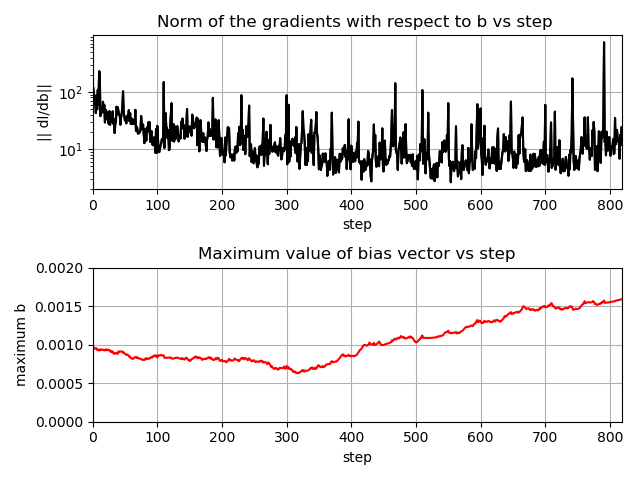
\includegraphics[width=0.8\linewidth]{ModRelu1.png}
  \caption{Norm of the gradients and maximum biases with steps(bias initialized in U[-0.01,0.001])}
  \label{fig_modrelu1}
\end{figure}

\begin{remark}
If b is positive and $|z| << b,$ then $|\frac{\partial f}{\partial z}|$ is extremly large and in fact NAN occurs. Even if $b>0$, but if $|z| \approx b,$ then $|\frac{\partial f}{\partial z}| \approx 1.5$
\end{remark}

\noindent To overcome this issue one may use $U[-l,-0.01], l > 0.01$ to initialize the nonlinearity biases with an additional threshold to the biases in the gradient decent process. namely one need to make sure that the biases not exceed zero or 0.001 in the gradient decent, otherwise similar unstability occurs in the training process. \\

\noindent If the initial state is initialize from the uniform distribution $U[-0.01,0.01]$, whether is it trainable or non trainable, network is not that sensitive to the initialization of the bias vector. As we seen from our experiments, the probability of getting NAN in his case was vary law and we never face to this issue while experiments.Figure \ref{fig_modrelu2} shows We found that the best performance occurs when the bias and the hidden state vector initialize from the uniform distribution $U[-0.01,0.01]$ and allow to be trainable.\\

\begin{figure}
\centering
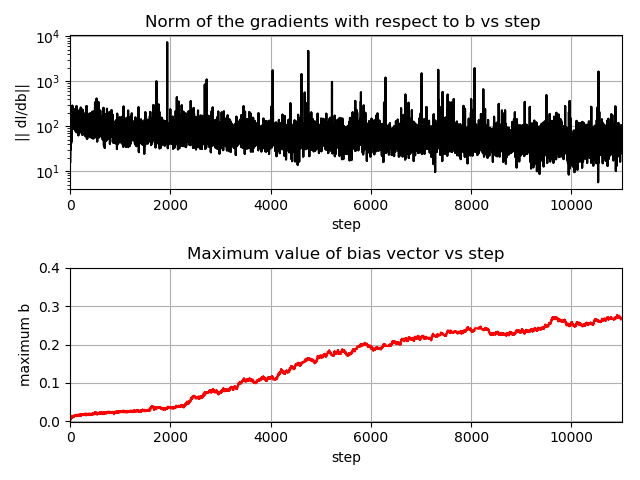
\includegraphics[width=0.8\linewidth]{ModRelu2.png}
  \caption{Norm of the gradients and maximum biases with steps(bias and initial state initialized in U[-0.01,0.01])}
  \label{fig_modrelu2}
\end{figure}

\noindent We closely experiment what happen to the bias vector in the training process and observe that the more biases are training towards the negative side, which we suspect this happens to avoid the singularity when the state become zero or close to zero up to machine precision. however best performance comes with the initialization that allows both negative and positive values to the bias vector even most of the biases training to be negative.  

\subsection{Update Scheme}

To update input-hidden, hidden-output parameters and all the biases, We follow the architecture described in \cite{Arjo16}. In this case we consider all complex numbers using real values considering the real and imaginary parts separately. We compute matrix vector product with real numbers as follows

\[ \begin{pmatrix}
\text{Re}(Vz)  \\
\text{Im}(Vz)  \end{pmatrix} =
\begin{pmatrix}
A & -B \\
B & A \end{pmatrix}
\begin{pmatrix}
\text{Re}(z)  \\
\text{Im}(z)  \end{pmatrix},
\]
\noindent where $V = A +iB$ and $z = x +iy,$ then $Vz = (Ax-By)+i(Ay+Bx).$ This allows us to update all the parameters using real valued operations.\\

\noindent Now for the update scheme on the skew-Hermitian matrix and the scaling matrix, we have to deal with the complex derivatives. When we consider the loss function as a function of the complex recurrent weight matrix with a range on the real-line, the loss function is nonholomorphic and thus not complex differentiable.   In order to compute the necessary gradients, Wirtinger calculus is required \cite{Kreutzdelgado09}.\\

\noindent In Wirtinger calculus, differentiable complex functions are viewed as differentiable functions over $\mathbb{R}^2$.  In particular, given a nonholomorphic function, $f: \mathbb{C} \to \mathbb{C}$, the differential $df$ is given by

\[
	df = \frac{\partial f}{\partial z}dz + \frac{\partial f}{\partial \overline{z}}d\overline{z},
\]

\noindent where $z := x + \it{i}y \in \mathbb{C}$ and $\overline{z} := x - \it{i}y \in \mathbb{C}$ is the conjugate, with Writinger derivatives given by  
\[
	\frac{\partial f}{\partial z} = \frac{1}{2}\left(\frac{\partial f}{\partial x} - \it{i}\frac{\partial f}{\partial y} \right) \qquad \text{and} \qquad \frac{\partial f}{\partial \overline{z}} = \frac{1}{2}\left(\frac{\partial f}{\partial x} + \it{i}\frac{\partial f}{\partial y}\right).
\]

\noindent Results from \cite{Kreutzdelgado09} allows us to implement gradient based update using $z \leftarrow z-2\, \frac{\partial f(z)}{\partial \overline{z}} \, ds$ where $ds$ can be interpreted as the learning rate. \\

\subsubsection{4.1.1 Learning the Skew-Hermitian Matrix and the Scaling Matrix}
\noindent We update $W$ through the skew-Hermitian parameterization matrix $A$. We compute the gradients using Cayley transform. The next Theorem is the complex version of the main theorem given in the scoRNN paper update scheme.\\

\noindent Notice that $D \in \mathbb{C}^{n \times n}$ is a diagonal matrix consisting of entries that are modulus one.  In particular, $D_{j,j} = e^{i\theta_j}$ where $0 \leq \theta_j \leq 2\pi$ for all $1 \leq j \leq n$ and $\it{i} = \sqrt{-1}$.  We can update the diagonal entries by performing gradient descent on the $\theta$ variables. The following theorem describes how to compute these gradients with respect to $\theta$. 

\begin{theorem}
\label{dldatheorem}
Let $L = L(W): \mathbb{C}^{n \times n}\rightarrow \mathbb{R}$ be some differentiable cost function for an RNN with the recurrent weight matrix $W$. Let $W = W(A,D) := (I+A)^{-1}(I-A)D$ where $A \in \mathbb{C}^{n \times n}$ is Skew-Hermitian and $D \in \mathbb{C}^{n \times n}$ is an unitary diagonal matrix. Then the gradient of $L = L(W(A,D))$ with respect to $\overline{A}$ is
$$ \frac{\partial L}{\partial \overline{A}} = C^T -\overline{C} $$
where $C:=((I+A)^{-1})^T \frac{\partial L}{\partial W}(D+W^T)$ and we have used the notation $\frac{\partial L}{\partial A}=\left[ \frac{\partial L}{\partial A_{i,j}} \right] \in \mathbb{C}^{n \times n}$ and $\frac{\partial L}{\partial W}=\left[ \frac{\partial L}{\partial W_{i,j}} \right] \in \mathbb{C}^{n \times n}$.
Furthermore, the gradient of $L = L(W(A,D))$ with respect to $\theta$ is given by
\[
	\frac{\partial L}{\partial \theta} = 2\text{Re}\left(\it{i} \left( \left(\frac{\partial L}{\partial W}^{T}Z \right)\odot I\right)d \right)
\]
where $d = \left[e^{\it{i}\theta_1}, e^{\it{i}\theta_2, ... e^{\it{i}\theta_n}} \right]^T$ is the diagonal vector of $D$ and $\odot$ denote the point-wise multiplication.
\end{theorem}


\noindent We use above theorem to update recurrent matrix. First we compute $\frac{\partial L}{\partial W},$ using standard backpropagation algorithm. Then using $\frac{\partial L}{\partial W},$ we compute $\frac{\partial L}{\partial A},$ and $\frac{\partial L}{\partial \theta},$ using the results given in the last two theorems. We then update the diagonal matrix by updating the vector $\theta$ by implementing an optimizer such as gradient descent.
\begin{align*}
 \theta^{(k+1)} &= \theta^{(k)} - \alpha \frac{\partial L}{\partial \theta^{(k)}}, \\
 D^{(k+1)}&=e^{i\theta^{(k+1)}},
\end{align*}
where $\alpha$ is the learning rate. Then we update the matrix $A$ similarly
$$ A^{(k+1)} =A^{(k)} -\beta \frac{\partial L}{\partial \overline{A}^{(k)}} ,$$
where $\beta$  is the learning rate. Now we construct the recurrent matrix using Cayley transform as
$$ W^{(k+1)}  = (I+A^{(k+1)})^{-1}(I-A^{(k+1)})D^{(k+1)}.$$
Notice that as $\frac{\partial L}{\partial \overline{A}}$ is skew-Hermitian, then $A^{(k+1)}$ will be skew-Hermitian, thus $W^{(k+1)}$ will be unitary up to machine precision.

  
\subsection{Initialization}

\noindent We use the same initialization used in \cite{kyle17} for the real part of the skew-hermitian matrix, while setting all the elements of the imaginary part being zero, which allow to learn from the gradient decent process. 

\begin{itemize}
\item Most importantly the initialization of the initial state effects the output state at the last time step to be either zero or close to zero, if we use zero initial state. therefore we initialize initial state with a uniform distribution, either $\mathcal{U}\left[ -0.01,0.01 \right]$ or $\mathcal{U}\left[ -\sqrt{\frac{3}{2N}},\sqrt{\frac{3}{2N}} \right],$ where $N$ is the number of hidden units.
\item We initialize $U$ and $V:$ input and output matrices with a uniform distribution \\ $\mathcal{U}\left[ - \frac{\sqrt{6}}{\sqrt{n_{in}+n_{out}}},\frac{\sqrt{6}}{\sqrt{n_{in}+n_{out}}} \right],$ as detailed in\cite{Glorot10}.
%\item For initializing the skew-hermitian matrix $A = B +\it{i}C,$ we initialize the skew symmetric matrix $B$ exactly similar to the scoRNN paper, while the symmetric matrix $C$ to be entirely zero matrix.
\item Initializing the diagonal weights for the scale diagonal matrix $D$, we use $\mathcal{U}\left[ 0,2\pi \right]$, which keeps the diagonal entries $D_{j,j}=e^{\it{i}\theta_j}$ over the complex unit circle.
\item The biases are initialized from $\mathcal{U}\left[ -0.01,0.01 \right].$


\end{itemize}

\section{Experiments}
\noindent In relation with the experiment, we compare the performance of the proposed method which we call scuRNN  with scoRNN, LSTM, restricted capacity uRNN and full-capacity uRNN. We follow the standard problems that commonly used to check the performance of RNNs in the past.  

\subsection{Pixel-By-Pixel MNIST}
This experiment deal with the well-known handwritten digit recognition task using the MNIST database \cite{LeCun}. We use 55,000 training set and 10,000 testing set for our classification task. We follow the procedure first suggested by\cite{Le15}, which feed the pixels of MNIST sequentially of length 784 as each image is $28 \times 28$ gray-scale image and obtain the target class label at the end between 0 and 9. We use RMSProp optimization algorithm, adagrad optimization algorithm and adam optimization algorithm with different learning rates for the skew-hermitian matrix parameters, the diagonal weights and other parameters. In the experiment we use RMSprop optimizer, Adam optimizer or adagrad optimizer with deferent learning rates for the diagonal weights updates.\\

\noindent Our experiment that uses $116$ hidden units, we use RMSprop optimization algorithm to update recurrent matrix with learning rate $10^{-4},$ adagrad optimization to update the diagonal matrix with learning rate $10^{-3}$, while other parameters trained using adam optimizer with learning rate $10^{-3}.$ Experiment uses 250 hidden units uses RMSprop optimization algorithm to update recurrent matrix with learning rate $10^{-5},$ adagrad optimization to update the diagonal matrix with learning rate $10^{-4}$, while other parameters trained using adam optimizer with learning rate $10^{-3}.$ All the machines are trained up to 70 epoch and the best test accuracy from the conclusion test accuracy at the end of each epoch is given in table \ref{t1}.

\noindent The Figure \ref{fig_mnist1} gives the test set accuracy in the first 70 epoch for the scuRNN (n=116), scuRNN (n=250), ScoRNN (n=170), LSTM (n=128), Restricted-capacity uRNN (n=512) and Full-capacity uRNN (n=116). here we adjust the number of hidden units n, so that they have approximately 16k number of trainable parameters except for the LSTM uses approximately 68k, trainable parameters. We used RMSprop optimizer for update skew-Hermitian matrix, with the learning rate $10^{-4}$ or $10^{-5},$ while adam optimizer for the in-out parameters and adagrad optimizer for the diagonal weights update with learning rate $10^{-3}$. Even though proposed method could not do better than the LSTM architecture, the 116 hidden unit scuRNN gives better results compare with the 170 hidden unit scoRNN architecture, and lot better compare with the 116 Full-capacity uRNN. For the 250 hidden units scuRNN gives same test accuracy as scoRNN with fewer number of hidden units. Also the proposed method gives competitive results compare with the restricted-capacity uRNN, with more than 4 times less number of hidden units.

\begin{table}[h]
\label{t1}
\begin{center}
\caption{Results for unpermuted pixel-by-pixel MNIST.}
\renewcommand{\arraystretch}{1.2}
\begin{tabular}{ | c | c | c | c |} 
\hline
\multicolumn{1}{|c|}{Model}  & 
\multicolumn{1}{|c|}{n} & 
\multicolumn{1}{|c|}{\# parameters}& 
\multicolumn{1}{|c|}{Test Accuracy}
\\ \hline
%%%%%%%%%%%%%%%%%%%%%%%%%%%%%%%%%%%%%%%%%%%%%%%%%%%%%%%%%%%%%%
scuRNN  
& \multicolumn{1}{|c|}{250} 
& \multicolumn{1}{|c|}{$\approx$ 69k}
& \multicolumn{1}{|c|}{0.983} 
\\\hline
%%%%%%%%%%%%%%%%%%%%%%%%%%%%%%%%%%%%%%%%%%%%%%%%%%%%%%%%%%%%%%
scuRNN  
& \multicolumn{1}{|c|}{116} 
& \multicolumn{1}{|c|}{$\approx$ 16k}
& \multicolumn{1}{|c|}{0.976} 
\\\hline
%%%%%%%%%%%%%%%%%%%%%%%%%%%%%%%%%%%%%%%%%%%%%%%%%%%%%%%%%%%%%%
scoRNN 
& \multicolumn{1}{|c|}{170} 
& \multicolumn{1}{|c|}{$\approx$ 16k}
& \multicolumn{1}{|c|}{0.973} 
\\\hline
%%%%%%%%%%%%%%%%%%%%%%%%%%%%%%%%%%%%%%%%%%%%%%%%%%%%%%%%%%%%%%
scoRNN 
& \multicolumn{1}{|c|}{360} 
& \multicolumn{1}{|c|}{$\approx$ 69k}
& \multicolumn{1}{|c|}{0.983} 
\\\hline
%%%%%%%%%%%%%%%%%%%%%%%%%%%%%%%%%%%%%%%%%%%%%%%%%%%%%%%%%%%%%%
$LSTM$  
& \multicolumn{1}{|c|}{128} 
& \multicolumn{1}{|c|}{$\approx$ 68k}
& \multicolumn{1}{|c|}{0.987} 
\\\hline
%%%%%%%%%%%%%%%%%%%%%%%%%%%%%%%%%%%%%%%%%%%%%%%%%%%%%%%%%%%%%%
$LSTM$  
& \multicolumn{1}{|c|}{256} 
& \multicolumn{1}{|c|}{$\approx$ 270k}
& \multicolumn{1}{|c|}{0.989} 
\\\hline
%%%%%%%%%%%%%%%%%%%%%%%%%%%%%%%%%%%%%%%%%%%%%%%%%%%%%%%%%%%%%%
Rest.-cap. uRNN  
& \multicolumn{1}{|c|}{512} 
& \multicolumn{1}{|c|}{$\approx$ 16k}
& \multicolumn{1}{|c|}{0.976} 
\\\hline
%%%%%%%%%%%%%%%%%%%%%%%%%%%%%%%%%%%%%%%%%%%%%%%%%%%%%%%%%%%%%%
Full-cap. uRNN  
& \multicolumn{1}{|c|}{116} 
& \multicolumn{1}{|c|}{$\approx$ 16k}
& \multicolumn{1}{|c|}{0.947} 
\\\hline
%%%%%%%%%%%%%%%%%%%%%%%%%%%%%%%%%%%%%%%%%%%%%%%%%%%%%%%%%%%%%%
Full-cap. uRNN  
& \multicolumn{1}{|c|}{512} 
& \multicolumn{1}{|c|}{$\approx$ 270k}
& \multicolumn{1}{|c|}{0.974} 
\\\hline
%%%%%%%%%%%%%%%%%%%%%%%%%%%%%%%%%%%%%%%%%%%%%%%%%%%%%%%%%%%%%%
\end{tabular}
\end{center}
\end{table}

\begin{figure}
\centering
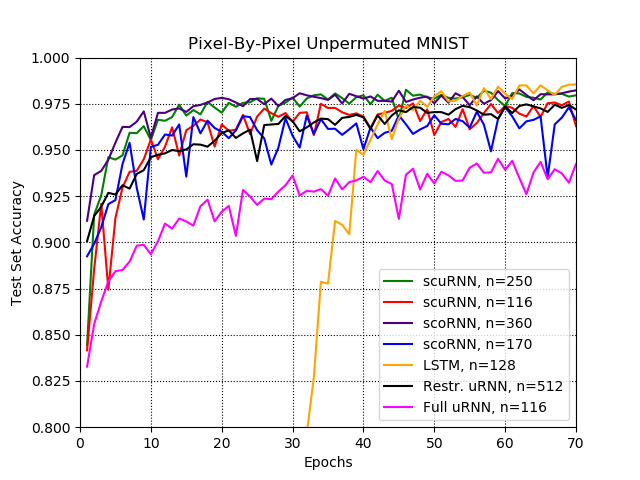
\includegraphics[width=0.8\linewidth]{Mnist_unpermuted.png}
  \caption{Pixel-by-Pixel Unpermute MNIST Results}
  \label{fig_mnist1}
\end{figure}

\subsection{Permuted Pixel-By-Pixel MNIST}
\noindent Here we use the same setup for the experiment as in the pixel-by-pixel MNIST given above, but use a fixed permutation to the pixels of MNIST to create many long term dependencies to  make the problem more harder. As in the unpermuted MNISt task all the machines are trained up to 70 epoch and the best test accuracy from the conclusion test accuracy at the end of each epoch is given in table \ref{t2}.\\


\begin{table}[h]
\label{t2}
\begin{center}
\caption{Results for permuted pixel-by-pixel MNIST.}
\renewcommand{\arraystretch}{1.2}
\begin{tabular}{ | c | c | c | c |} 
\hline
\multicolumn{1}{|c|}{Model}  & 
\multicolumn{1}{|c|}{n} & 
\multicolumn{1}{|c|}{\# parameters}& 
\multicolumn{1}{|c|}{Test Accuracy} 
\\ \hline
%%%%%%%%%%%%%%%%%%%%%%%%%%%%%%%%%%%%%%%%%%%%%%%%%%%%%%%%%%%%%%
scuRNN  
& \multicolumn{1}{|c|}{250} 
& \multicolumn{1}{|c|}{$\approx$ 69k}
& \multicolumn{1}{|c|}{0.962} 
\\\hline
%%%%%%%%%%%%%%%%%%%%%%%%%%%%%%%%%%%%%%%%%%%%%%%%%%%%%%%%%%%%%%
scuRNN  
& \multicolumn{1}{|c|}{170} 
& \multicolumn{1}{|c|}{$\approx$ 33k}
& \multicolumn{1}{|c|}{0.953} 
\\\hline
%%%%%%%%%%%%%%%%%%%%%%%%%%%%%%%%%%%%%%%%%%%%%%%%%%%%%%%%%%%%%%
scuRNN  
& \multicolumn{1}{|c|}{116} 
& \multicolumn{1}{|c|}{$\approx$ 16k}
& \multicolumn{1}{|c|}{0.949} 
\\\hline
%%%%%%%%%%%%%%%%%%%%%%%%%%%%%%%%%%%%%%%%%%%%%%%%%%%%%%%%%%%%%%
scoRNN 
& \multicolumn{1}{|c|}{360} 
& \multicolumn{1}{|c|}{$\approx$ 69k}
& \multicolumn{1}{|c|}{0.962} 
\\\hline
%%%%%%%%%%%%%%%%%%%%%%%%%%%%%%%%%%%%%%%%%%%%%%%%%%%%%%%%%%%%%%
scoRNN 
& \multicolumn{1}{|c|}{170} 
& \multicolumn{1}{|c|}{$\approx$ 16k}
& \multicolumn{1}{|c|}{0.943} 
\\\hline
%%%%%%%%%%%%%%%%%%%%%%%%%%%%%%%%%%%%%%%%%%%%%%%%%%%%%%%%%%%%%%
$LSTM$  
& \multicolumn{1}{|c|}{128} 
& \multicolumn{1}{|c|}{$\approx$ 68k}
& \multicolumn{1}{|c|}{0.920} 
\\\hline
%%%%%%%%%%%%%%%%%%%%%%%%%%%%%%%%%%%%%%%%%%%%%%%%%%%%%%%%%%%%%%
$LSTM$  
& \multicolumn{1}{|c|}{256} 
& \multicolumn{1}{|c|}{$\approx$ 270k}
& \multicolumn{1}{|c|}{0.929} 
\\\hline
%%%%%%%%%%%%%%%%%%%%%%%%%%%%%%%%%%%%%%%%%%%%%%%%%%%%%%%%%%%%%%
Rest.-cap. uRNN  
& \multicolumn{1}{|c|}{512} 
& \multicolumn{1}{|c|}{$\approx$ 16k}
& \multicolumn{1}{|c|}{0.945} 
\\\hline
%%%%%%%%%%%%%%%%%%%%%%%%%%%%%%%%%%%%%%%%%%%%%%%%%%%%%%%%%%%%%%
Full-cap. uRNN  
& \multicolumn{1}{|c|}{116} 
& \multicolumn{1}{|c|}{$\approx$ 16k}
& \multicolumn{1}{|c|}{0.925} 
\\\hline
%%%%%%%%%%%%%%%%%%%%%%%%%%%%%%%%%%%%%%%%%%%%%%%%%%%%%%%%%%%%%%
Full-cap. uRNN  
& \multicolumn{1}{|c|}{512} 
& \multicolumn{1}{|c|}{$\approx$ 270k}
& \multicolumn{1}{|c|}{0.947} 
\\\hline
%%%%%%%%%%%%%%%%%%%%%%%%%%%%%%%%%%%%%%%%%%%%%%%%%%%%%%%%%%%%%%
\end{tabular}
\end{center}
\end{table}
\vspace{-0.2in}
\begin{figure}
\centering
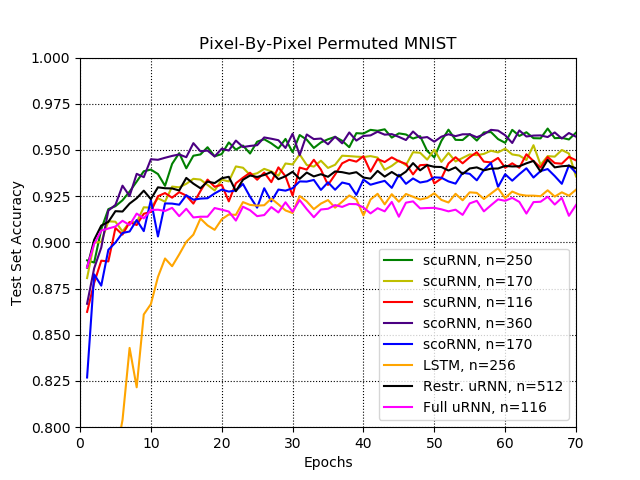
\includegraphics[width=0.8\linewidth]{Mnist_permuted.png}
  \caption{Pixel-by-Pixel permute MNIST Results}
  \label{fig_mnist2}
\end{figure}

\noindent Figure \ref{fig_mnist2} gives the test set accuracy in the first 70 epoch for the scuRNN (n=116, n=170 and n=250), scoRNN (n=170 and n=360), LSTM (n=128 and n=256), Restricted-capacity uRNN (n=512) and Full-capacity uRNN (n=116 and n=512). For complex scoRNN with 116 hidden units, we used RMSprop optimizer for update skew-Hermitian matrix, with the learning rate $10^{-4},$ while Adam optimizer for the in-out parameters and adagrad optimizer for the diagonal weights update with learning rate $10^{-3}$. For complex scoRNN with 170 hidden units, we used RMSprop optimizer for update skew-Hermitian matrix, with the learning rate $10^{-5},$ while adam optimizer for the in-out parameters and adagrad optimizer for the diagonal weights update with learning rate $10^{-3}$. In this task scuRNN achieves 96.2\% with 250 hidden units which passes all the other uRNN architectures and LSTM while similar accuracy as in the scoRNN with 360 hidden units. \\

\subsection{Copying Problem}
\noindent Here we describe copying problem first proposed by \cite{Arjo16} and used by \cite{kyle17}. Copying problem uses to check the ability of an RNN to reproduce a sequence seen many time steps earlier. We use the setup described in \cite{kyle17}, which we used 10 input classes denoted by the digits 0-9, where 0 used as a 'blank' class and 9 used as a 'marker' class. The RNN need to remember 10 syllables, which are uniformly sampled from classes 1-8, over a sequence of length $T+20.$ The goal of the network is reproduce ten syllables after T time steps. The expected categorical cross entropy for this task is $\frac{10 \log (8)}{T+20}.$\\

\noindent For our experiment we adjust the number of hidden units of each network to match the number of parameters to be 22k approximately. As a result we train an LSTM with $n = 68,$ a restricted-capacity uRNN with $n=470,$ a full-capacity uRNN with $n= 128,$ a scoRNN with $n=190,$ and a scuRNN with $n=130$.\\

\noindent For the T=1000 task we use RMSprop optimizer for update skew-Hermitian matrix, with the learning rate $10^{-4},$ while Adam optimizer for the in-out parameters with learning rate $10^{-3}$ and adagrad optimizer for the diagonal weights update with learning rate $10^{-4}$.For the T=2000 task we use RMSprop optimizer for update skew-Hermitian matrix and in-out parameters with the learning rate $10^{-3},10^{-3}$ respectively  while Adam optimizer for the diagonal weights update with learning rate $10^{-4}$.

\noindent Figure \ref{fig_copying} compares each model's for T=1000 and T=2000. The base line cross entropy given in the dash line. In the both problems , the restricted-capacity uRNN and LSTM converging rapidly to the base line solution and fail to converge to zero cross entropy. For T =1000 test problem, the full-capacity uRNN, scoRNN and scuRNN converges quickly to zero cross entropy solution. For T=2000 scuRNN converges faster than all the other networks, even unable to bypass the baseline strategy entirely.\\

\begin{figure}
    \centering
    \subfloat{{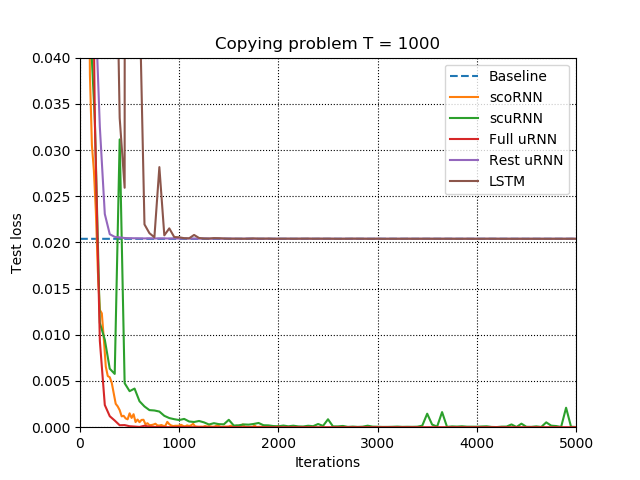
\includegraphics[width=7cm]{Copying_1000} }}%
    \qquad
    \subfloat{{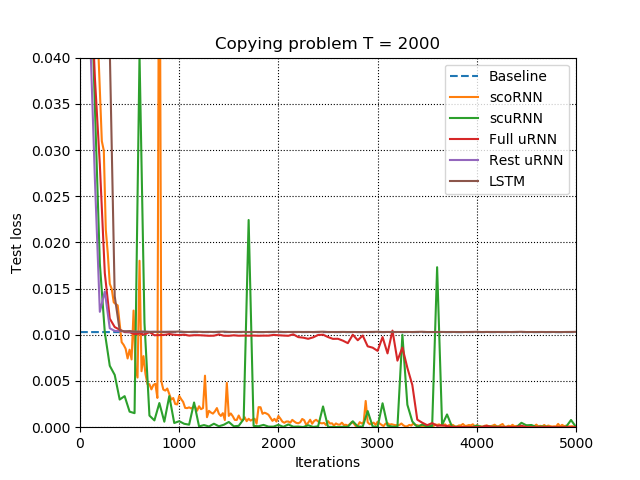
\includegraphics[width=7cm]{Copying_T_2000} }}%
    \caption{Cross entropy of each machine on the copying problem with T = 1000 ( left) and T=2000 ( right).}%
    \label{fig_copying}%
\end{figure}


\subsection{Adding Problem}

\noindent Here we describe adding problem first proposed by \cite{Arjo16} and used by \cite{kyle17}. In this problem input vector is a two sequences of length $T$. The first sequence is sampled from $\mathcal{U}\left[0,1\right).$ The second sequence consist exactly two entries being 1, and the remaining entries are 0. The first 1 in the second sequence is located in the first half of the sequence uniformly while the second 1 is locates again uniformly at random in the other half $\left[ \frac T 2 , T \right)$ of the sequence. The task of the network is to predict the sum of the two numbers from the first sequence that marked as 1 in the second sequence. Models are trained to minimize the Mean Square Error (MSE). The baseline for the task is 0.167 which is the expected MSE for a model that always output one, regardless of the sequence.\\

\noindent We experiment with sequence length 200 and 400, and uses a training set size of 100,000 and testing set of 10,000 as in \cite{kyle17}, also each network uses different number of hidden units, for the purpose of matching the number of trainable parameters to be 14k. We use $N = 116$ for the scuRNN, $N= 170$ for the scoRNN, $N= 60$ for LSTM, $N = 120$ for the full-capacity uRNN, and $N=950$ for the restricted-capacity uRNN.\\

\noindent Figure \ref{fig_addins_200} indicate the test set MSE for each architecture on the adding problem with sequence length 200. All the architectures get their start near or at the base line and keep dropping to the zero by the number of epoch getting higher. Most impotently even the proposed method MSE curve move up and down compare with the scuRNN architecture, it lies below the other complex valued architectures.\\



\begin{figure}
\centering
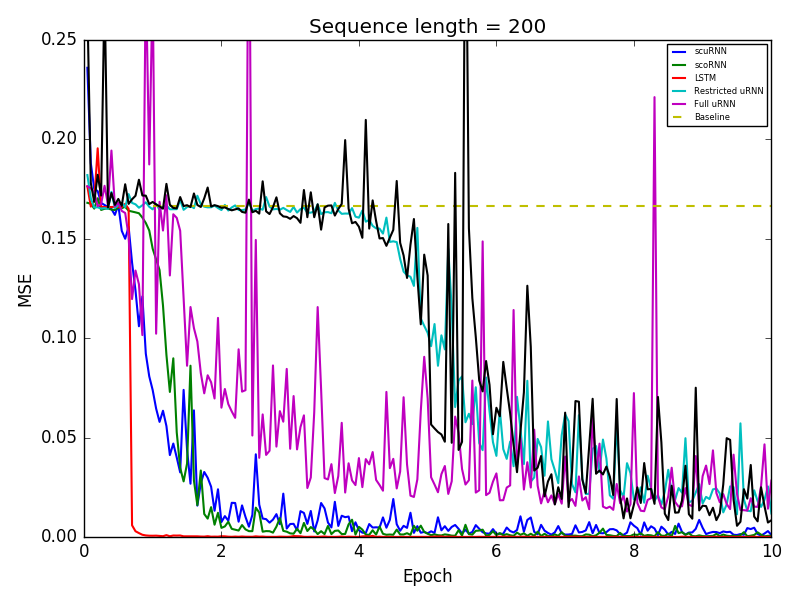
\includegraphics[width=0.8\linewidth]{adding_200.png}
  \caption{Test set MSE of each machine on adding problem with sequence length 200.}
  \label{fig_addins_200}
\end{figure}

\noindent Figure \ref{fig_adding_400} indicate the test set MSE for each architecture on the adding problem with sequence length 400. Curves behave very closely with the sequence length 200. As always LSTM drops fist below the base line, and comparably better than other uRNN architectures in the filed. When we compare with the scoRNN architecture, proposed method more irregular descent curve.\\

\noindent Figure \ref{fig_adding_750} indicate the test set MSE for each architecture on the adding problem with sequence length 750. LSTM drops fist below the base line,and then scuRNN drops slightly below the baseline before other architecture. Even though scoRNN architecture bypass the scuRNN around 5th epoch and having more irregular curve, comparably act better than the other uRNN networks. We suspect that introducing complex valued argument makes the descent curve more osculating than the real valued case. \\

\begin{figure}
\centering
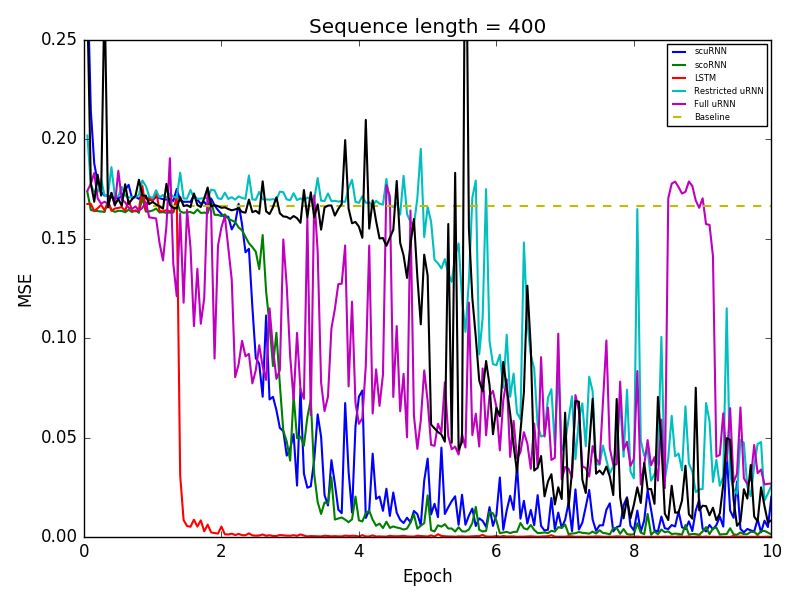
\includegraphics[width=0.8\linewidth]{adding_400.png}
  \caption{Test set MSE of each machine on adding problem with sequence length 400.}
  \label{fig_adding_400}
\end{figure}

\begin{figure}
\centering
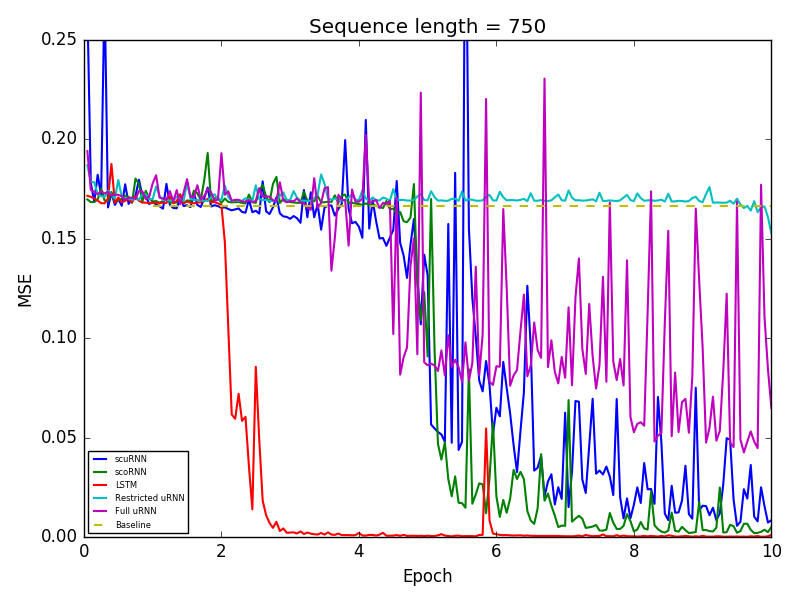
\includegraphics[width=0.8\linewidth]{adding_750.png}
  \caption{Test set MSE of each machine on adding problem with sequence length 400.}
  \label{fig_adding_750}
\end{figure}

\subsection{TIMIT Speech Dataset}
We test our scuRNN model on audio data using TIMIT data base \cite{garafolo93}.We use the same setup discribed by \cite{kyle17} that uses only he core test set, the data set consisting of 3,96 training set and 192 testing set and 400 evaluation audio files. Audio files were down sampled as detailed in \cite{Wisdom16}. For experiment on TIMIT daa set with scuRNN architecture with 128,190 ans 258 hidden units to match the number of parameters 83k,135k and 200k perspectively.Best optimizers and bes learning rates ned to include here.\\

\noindent Following table \ref{t3} includes the  mean square error (MSE) on validation and evaluation date sets for scuRNN, scoRNN, LSTM, R. uRNN ( restricted capacity uRNN) and F.uRNN ( Full-capacity uRNN) architectures for the comparison. Here MSE obtained using the predicted and actual log magnitudes of the next time frame over the entire sequence.

\begin{table}[h]
\label{t3}
\begin{center}
\caption{Results for TIMIT speech set. Evaluaion based on MSE}
\renewcommand{\arraystretch}{1.2}
\begin{tabular}{ | c | c | c | c |c |} 
\hline
\multicolumn{1}{|c|}{Model}  & 
\multicolumn{1}{|c|}{n} & 
\multicolumn{1}{|c|}{\# PARAMS}& 
\multicolumn{1}{|c|}{VALID MSE} &
\multicolumn{1}{|c|}{EVAL. MSE}
\\ \hline
%%%%%%%%%%%%%%%%%%%%%%%%%%%%%%%%%%%%%%%%%%%%%%%%%%%%%%%%%%%%%%
scuRNN  
& \multicolumn{1}{|c|}{128} 
& \multicolumn{1}{|c|}{$\approx$ 83k}
& \multicolumn{1}{|c|}{4.06}
& \multicolumn{1}{|c|}{3.78}
\\\hline
%%%%%%%%%%%%%%%%%%%%%%%%%%%%%%%%%%%%%%%%%%%%%%%%%%%%%%%%%%%%%%
scuRNN  
& \multicolumn{1}{|c|}{190} 
& \multicolumn{1}{|c|}{$\approx$ 135k}
& \multicolumn{1}{|c|}{2.91}
& \multicolumn{1}{|c|}{2.68}
\\\hline
%%%%%%%%%%%%%%%%%%%%%%%%%%%%%%%%%%%%%%%%%%%%%%%%%%%%%%%%%%%%%%
scuRNN  
& \multicolumn{1}{|c|}{258} 
& \multicolumn{1}{|c|}{$\approx$ 200k}
& \multicolumn{1}{|c|}{2.15}
& \multicolumn{1}{|c|}{1.99}
\\\hline
%%%%%%%%%%%%%%%%%%%%%%%%%%%%%%%%%%%%%%%%%%%%%%%%%%%%%%%%%%%%%%
scoRNN  
& \multicolumn{1}{|c|}{224} 
& \multicolumn{1}{|c|}{$\approx$ 83k}
& \multicolumn{1}{|c|}{9.26}
& \multicolumn{1}{|c|}{8.50}
\\\hline
%%%%%%%%%%%%%%%%%%%%%%%%%%%%%%%%%%%%%%%%%%%%%%%%%%%%%%%%%%%%%%
scoRNN 
& \multicolumn{1}{|c|}{322} 
& \multicolumn{1}{|c|}{$\approx$ 135k}
& \multicolumn{1}{|c|}{8.48} 
& \multicolumn{1}{|c|}{7.82}
\\\hline
%%%%%%%%%%%%%%%%%%%%%%%%%%%%%%%%%%%%%%%%%%%%%%%%%%%%%%%%%%%%%%
scoRNN 
& \multicolumn{1}{|c|}{425} 
& \multicolumn{1}{|c|}{$\approx$ 200k}
& \multicolumn{1}{|c|}{7.97}
& \multicolumn{1}{|c|}{7.36}
\\\hline
%%%%%%%%%%%%%%%%%%%%%%%%%%%%%%%%%%%%%%%%%%%%%%%%%%%%%%%%%%%%%%
$LSTM$  
& \multicolumn{1}{|c|}{84} 
& \multicolumn{1}{|c|}{$\approx$ 83k}
& \multicolumn{1}{|c|}{15.42} 
& \multicolumn{1}{|c|}{14.30}
\\\hline
%%%%%%%%%%%%%%%%%%%%%%%%%%%%%%%%%%%%%%%%%%%%%%%%%%%%%%%%%%%%%%
$LSTM$  
& \multicolumn{1}{|c|}{120} 
& \multicolumn{1}{|c|}{$\approx$ 135k}
& \multicolumn{1}{|c|}{13.93} 
& \multicolumn{1}{|c|}{12.62}
\\\hline
%%%%%%%%%%%%%%%%%%%%%%%%%%%%%%%%%%%%%%%%%%%%%%%%%%%%%%%%%%%%%%
$LSTM$  
& \multicolumn{1}{|c|}{158} 
& \multicolumn{1}{|c|}{$\approx$ 200k}
& \multicolumn{1}{|c|}{13.66} 
& \multicolumn{1}{|c|}{12.62}
\\\hline
%%%%%%%%%%%%%%%%%%%%%%%%%%%%%%%%%%%%%%%%%%%%%%%%%%%%%%%%%%%%%%
R.uRNN  
& \multicolumn{1}{|c|}{158} 
& \multicolumn{1}{|c|}{$\approx$ 83k}
& \multicolumn{1}{|c|}{15.57} 
& \multicolumn{1}{|c|}{18.51}
\\\hline
%%%%%%%%%%%%%%%%%%%%%%%%%%%%%%%%%%%%%%%%%%%%%%%%%%%%%%%%%%%%%%
R.uRNN  
& \multicolumn{1}{|c|}{256} 
& \multicolumn{1}{|c|}{$\approx$ 135k}
& \multicolumn{1}{|c|}{15.90} 
& \multicolumn{1}{|c|}{15.31}
\\\hline
%%%%%%%%%%%%%%%%%%%%%%%%%%%%%%%%%%%%%%%%%%%%%%%%%%%%%%%%%%%%%%
R.uRNN  
& \multicolumn{1}{|c|}{378} 
& \multicolumn{1}{|c|}{$\approx$ 200k}
& \multicolumn{1}{|c|}{16.00} 
& \multicolumn{1}{|c|}{15.15}
\\\hline
%%%%%%%%%%%%%%%%%%%%%%%%%%%%%%%%%%%%%%%%%%%%%%%%%%%%%%%%%%%%%%
F.uRNN  
& \multicolumn{1}{|c|}{128} 
& \multicolumn{1}{|c|}{$\approx$ 83k}
& \multicolumn{1}{|c|}{15.07}
& \multicolumn{1}{|c|}{14.58}
\\\hline
%%%%%%%%%%%%%%%%%%%%%%%%%%%%%%%%%%%%%%%%%%%%%%%%%%%%%%%%%%%%%%
F.uRNN  
& \multicolumn{1}{|c|}{192} 
& \multicolumn{1}{|c|}{$\approx$ 135k}
& \multicolumn{1}{|c|}{15.10} 
& \multicolumn{1}{|c|}{14.50}
\\\hline
%%%%%%%%%%%%%%%%%%%%%%%%%%%%%%%%%%%%%%%%%%%%%%%%%%%%%%%%%%%%%%
F.uRNN  
& \multicolumn{1}{|c|}{256} 
& \multicolumn{1}{|c|}{$\approx$ 200k}
& \multicolumn{1}{|c|}{14.96} 
& \multicolumn{1}{|c|}{14.69}
\\\hline
%%%%%%%%%%%%%%%%%%%%%%%%%%%%%%%%%%%%%%%%%%%%%%%%%%%%%%%%%%%%%%
\end{tabular}
\end{center}
\end{table}


\section{Conclusion}
\noindent In this proposed RNN architecture, we presented a new parametrization of the  unitary transition matrix using scaled Cayley transform. In contrast with other proposed URNN architectures this methods keeps the unitary properties of the recurrent matrix up to machine precision over the entire training process. Results from the MNIST data set with permuted and unpermuted experiments and the adding problem demonstrate the better or competiive results with the scoRNN architecture and recent URNN architectures.\\

\section{Appendix}

%\begin{theorem}
%The differential $df$ of a non-holomorphic function $f(z):\mathbb{A}\mapsto \mathbb{R}$ with $\mathbb{A} \subset \mathbb{C}$ can be expressed as 
%\begin{gather}
%\label{eqdf}
%df = 2\text{Real} \left( \frac{\partial f(z)}{\partial z} dz \right)  = 2\text{Real} \left( \frac{\partial f(z)}{\partial \overline{z}} d\overline{z} \right),
%\end{gather}
%and is equivalent to $$dF = \frac{\partial F(x,y)}{\partial x} dx + \frac{\partial F(x,y)}{\partial y}dy,$$ where $f(z)= F(x,y) = U(x,y)+\it{i} V(x,y). $
%\end{theorem}
%\noindent Now using above definition one can easily see the following result.
%\begin{theorem}
%The differential $df$ of a non-holomorphic function $f(z):\mathbb{A}\mapsto \mathbb{R}$ with $\mathbb{A} \subset \mathbb{C}$ can be expressed as 
%\begin{gather}
%\label{eqdf}
%df = 2\text{Real} \left( \frac{\partial f(z)}{\partial z} dz \right)  = 2\text{Real} \left( \frac{\partial f(z)}{\partial \overline{z}} d\overline{z} \right),
%\end{gather}
%and is equivalent to $$dF = \frac{\partial F(x,y)}{\partial x} dx + \frac{\partial F(x,y)}{\partial y}dy,$$ where $f(z)= F(x,y) = U(x,y)+\it{i} V(x,y). $
%\end{theorem}
%\noindent In order to find the stationary points $z$ of $f(z)$, one need to detect the points that vanishes the differential $df$. Note that if $\frac{\partial f(z)}{\partial z} = 0,$ then by the above theorem, we have $df =0.$ Conversely, $df$ and thus $dF$ will be zero if both partial derivatives of $F(x,y)$ with respect to $x$ and $y$ are zero. Now since we have the relation $$\frac{\partial f(z)}{\partial z} dz = \frac 1 2 \left[\frac{\partial U(x,y)}{\partial x} - \it{i}\frac{\partial U(x,y)}{\partial y}  \right](dx+\it{i}dy) $$
%which leads to $\frac{\partial f(z)}{\partial z} = 0.$ Altogether, we have that, the differential $df$ of a real-valued function $f(z):\mathbb{A}\mapsto \mathbb{R}$ with complex argument $z \in \mathbb{A}\subset \mathbb{C}$ vanishes if and only if the Writinger derivative is zero.\\

%\noindent Our goal is to use Wirtinger calculus to  implement gradient based algorithm that optimize an objective function which is not analytic. We can optimize $dz$ in the differential expression~(\ref{eqdf}) using the following result.\\

%\begin{theorem}
%The steepest ascent of a real valued function $f(z):\mathbb{A} \mapsto \mathbb{R}$ with complex valued argument $z \in \mathbb{A} \subset \mathbb{C}$ is obtained for
%$$ dz = \frac{\partial f(z)}{\partial \overline{z}} \,ds, $$
%where $ds$ is a real-valued differential. Thus, the steepest ascent points to the direction of $\frac{\partial f(z)}{\partial \overline{z}}.$  
%\end{theorem}
%\begin{proof}
%We consider $df$ from equation (\ref{eqdf}), and use Cauchy–Schwarz inequality to obtain, 
%\begin{align*}
%df &= 2\text{Real} \left( \frac{\partial f(z)}{\partial z} dz \right)
%   = 2\text{Real} \left[ \left\langle dz,\overline{\frac{\partial f}{\partial z}} \right\rangle \right] \\
%   &\leq \left\vert \left\langle dz,\overline{\frac{\partial f}{\partial z}} \right\rangle \right\vert \leq |dz|\, \left\vert \overline{\frac{\partial f}{\partial z}} \right\vert = |dz|\, \left\vert \frac{\partial f}{\partial \overline{z}} \right\vert.
%\end{align*}
%\noindent Observe that equality in the above relationship holds if $dz$ and $\frac{\partial f}{\partial \overline{z}}$ have the same direction.  Hence, $dz$ has to be a scaled version of $\frac{\partial f(z)}{\partial \overline{z}},$ and thus $df$ is maximized in the direction of $\frac{\partial f(z)}{\partial \overline{z}}$. Thus $dz = \frac{\partial f(z)}{\partial \overline{z}} \,ds$ as desired.   
%\end{proof}

Proof of the theorem include main update scheme
\begin{proof}
We compute the partial derivative $\frac{\partial L}{\partial A}$ and use the property $\frac{\partial L}{\partial \overline{A}}= \overline{\frac{\partial L}{\partial A}}$, to obtain the required result. Let $Z := (I+A)^{-1}(I-A)$, then $W = ZD$. We consider the $(i,j)$ entry of $\frac{\partial L}{\partial A}.$ Now taking the derivative with respect to $A_{i,j},$ where $i \neq j$ we obtain:

\begin{align*}
& \frac{\partial L}{\partial A_{i,j}} = \sum_{k,l = 1}^{n} \left(\frac{\partial L}{\partial W_{k, l}}
\frac{\partial W_{k, l}}{\partial A_{i,j}} 
+ \frac{\partial L}{\partial \overline{W}_{k,l}} \frac{\partial \overline{W}_{k, l}}{\partial A_{i,j}}\right) \\
 &= \sum_{k = 1}^{n} \left(\frac{\partial L}{\partial W_{k, j}}
D_{l,l}\frac{\partial Z_{k, l}}{\partial A_{i,j}}\right) 
+ \sum_{k = 1}^{n} \left( \frac{\partial L}{\partial \overline{W}_{k,l}} \overline{D_{j,j}}\frac{\partial \overline{Z_{k, l}}}{\partial A_{i,j}}\right) \\
 &= \underbrace{\it{tr}\left[\left(\frac{\partial L}{\partial W} D\right)^T \frac{\partial Z}{\partial A_{i,j}}\right]}_{\text{I}}
+ \underbrace{\it{tr}\left[\left(\overline{\frac{\partial L}{\partial W} D}\right)^T \left(\overline{\frac{\partial Z}{\partial \overline{A_{i,j}}}}\right)\right]}_{\text{II}}. 
\end{align*}

\noindent Consider the notation $A = X +\it{i}Y,$ where $X,Y \in \mathbb{R}^{n \times n}.$ So the identity $(I+A)Z = I-A$ become $(I+X+\it{i}Y)Z = I-X-\it{i}Y.$ Taking the derivatives with respect to $X_{i,j}$ and $Y_{i,j}$ we have:
\begin{gather}
\frac{\partial Z}{\partial X_{i,j}} = -(I+A)^{-1}\left( \frac{\partial X}{\partial X_{i,j}} + \frac{\partial X}{\partial X_{i,j}} Z \right),\\
\frac{\partial Z}{\partial Y_{i,j}} = -\it{i}(I+A)^{-1}\left( \frac{\partial Y}{\partial Y_{i,j}} + \frac{\partial Y}{\partial Y_{i,j}} Z \right).
\end{gather}

\noindent Now let $E_{i,j}$ denote the matrix whose $(i,j)$ entry is 1 with all other being zero. Since $X$ is Skew-symmetric we have $\frac{\partial X}{\partial X_{i,j}} = E_{i,j}-E_{j,i}.$ Similarly, since $Y$ is symmetric we have $\frac{\partial Y}{\partial Y_{i,j}} = E_{i,j}+E_{j,i}.$ Using above derivatives with the properties we obtain:

\begin{align*}
\frac{\partial Z}{\partial A_{i,j}} &= \frac{1}{2}\left( \frac{\partial Z}{\partial X_{i,j}} -\it{i} \frac{\partial Z}{\partial Y_{i,j}}\right)\\
&= \frac{1}{2}\left[ -(I+A)^{-1} \frac{\partial X}{\partial X_{i,j}} (I+ Z)\right]\\
&-\frac{1}{2}\left[\it{i}(-\it{i})(I+A)^{-1} \frac{\partial Y}{\partial Y_{i,j}} (I+ Z) \right]\\
&= \frac{1}{2}\left[ -(I+A)^{-1} \left(\frac{\partial X}{\partial X_{i,j}} + \frac{\partial Y}{\partial Y_{i,j}}\right)(I+ Z) \right]\\
&= -(I+A)^{-1} E_{i,j}(I+Z).
\end{align*}
\noindent Here last step obtained using Skew-symmetric property of $X$ and symmetric properties of $Y$. Following same argument one obtain:

\begin{align*}
\frac{\partial \overline{Z}}{\partial A_{i,j}} 
&= \left(\overline{\frac{\partial Z}{\partial \overline{A_{i,j}}}}\right)=\frac{1}{2}\overline{\left( \frac{\partial Z }{\partial X_{i,j}} -\it{i} \frac{\partial Z}{\partial Y_{i,j}}\right)}\\
&= \overline{(I+A)^{-1} E_{j,i}(I+Z)}.
\end{align*}
Finally we compute trace given in equation I as follows:
\begin{align*}
\text{I} &= \it{tr}\left[\left(\frac{\partial L}{\partial W} D\right)^T \frac{\partial Z}{\partial A_{i,j}}\right]\\
&= -\it{tr}\left[\left(\frac{\partial L}{\partial W} D\right)^T (I+A)^{-1}(E_{i,j}+E_{i,j}Z) \right]\\
&= -\it{tr}\left[\left(\frac{\partial L}{\partial W} D\right)^T (I+A)^{-1}E_{i,j}\right]\\
&-\it{tr}\left[\left(\frac{\partial L}{\partial W} D\right)^T (I+A)^{-1}E_{i,j}Z\right]\\
&= -\left[\left(\left(\frac{\partial L}{\partial W} D\right)^T (I+A)^{-1}\right)^T\right]_{i,j}\\
&-\left[\left(\left(\frac{\partial L}{\partial W} D\right)^T (I+A)^{-1}\right)^T Z^T\right]_{i,j}\\
&= -\left[\left(\left(\frac{\partial L}{\partial W} D\right)^T (I+A)^{-1}\right)^T(I+Z^T)\right]_{i,j}\\
&=-\left[ ((I+A)^{-1})^T \frac{\partial L}{\partial W} (D +DZ^T)\right]_{i,j}  \\
&= -\left[ \left((I+A)^{-1}\right)^T \frac{\partial L}{\partial W}(D+W^T)\right]_{i,j}.
\end{align*}
\noindent Similar approach gives the second equation II as follows:
\begin{align*}
\text{II} &= \it{tr}\left[\overline{\left(\frac{\partial L}{\partial W} D\right)}^T \overline{\frac{\partial Z}{\partial \overline{A_{i,j}}}}\right]\\
&= \it{tr}\left[\overline{\left(\frac{\partial L}{\partial W} D\right)^T} \overline{(I+A)^{-1}}\overline{(E_{j,i}+E_{j,i}Z)} \right]\\
&= \it{tr}\left[\overline{\left(\frac{\partial L}{\partial W} D\right)}^T \overline{(I+A)^{-1}} \overline{E_{j,i}}  \right] \\ 
&+ \it{tr}\left[\overline{\left(\frac{\partial L}{\partial W} D\right)}^T \overline{(I+A)^{-1}} \overline{E_{j,i}Z}  \right]\\
&= \left[\overline{\left(\frac{\partial L}{\partial W} D\right)}^T \overline{(I+A)^{-1}} \right]_{i,j}  
+ \left[\overline{Z} \overline{\left(\frac{\partial L}{\partial W} D\right)}^T \overline{(I+A)^{-1}}\right]_{i,j}\\
&=\left[ (I+\overline{Z}) \overline{\left(\frac{\partial L}{\partial W} D\right)}^T \overline{(I+A)^{-1}} \right]_{i,j} \\
&= \left[ \overline{(D^T+W)} \overline{\frac{\partial L}{\partial W}}^T\overline{(I+A)^{-1}}\right]_{i,j}.
\end{align*}
Now by the definition of $C$, we can see that 
$$\frac{\partial L}{\partial A} = \overline{C}^T -C. $$
Therefore the desired result follows as
$$ \frac{\partial L}{\partial \overline{A}} = \overline{\frac{\partial L}{\partial A}} = = C^T -\overline{C}. $$

Consider the backpropagating on the $\theta_j$ variables for all $1 \leq j \leq n$  

\begin{align*}
\frac{\partial L}{\partial \theta_{j}} &= \sum_{k = 1}^{n} \left(\frac{\partial L}{\partial W_{k, j}}
\frac{\partial W_{k, j}}{\partial \theta_j} 
+ \frac{\partial L}{\partial \overline{W}_{k,j}} \frac{\partial \overline{W}_{k, j}}{\partial \theta_j}\right) \\
 &= \sum_{k = 1}^{n} \left(\frac{\partial L}{\partial W_{k, j}}
\frac{\partial Z_{k, j}D_{j,j}}{\partial \theta_j} 
+ \frac{\partial L}{\partial \overline{W}_{k,j}} \frac{\partial \overline{Z_{k, j}D_{j,j}}}{\partial \theta_j}\right) \\
 &= \sum_{k = 1}^{n} \left(\frac{\partial L}{\partial W_{k, j}}
Z_{k, j}\frac{\partial e^{\it{i}\theta_j}}{\partial \theta_j} 
+ \frac{\partial L}{\partial \overline{W}_{k,j}} \overline{Z_{k, j}}\frac{\partial e^{-\it{i}\theta_j}}{\partial \theta_j}\right) \\
 &= \it{i}\sum_{k = 1}^{n} \frac{\partial L}{\partial W_{k, j}}Z_{k, j}\it{i}D_{j,j} -\it{i}\sum_{k = 1}^{n} \frac{\partial L}{\partial \overline{W}_{k,j}}\overline{Z}
_{k,j}\overline{D}_{j,j}
\end{align*}

\noindent where $Z := \left(I + A\right)^{-1}\left(I - A\right)$.  Since this holds for all $0 \leq j \leq n$ we have

\begin{align*}
\frac{\partial L}{\partial \theta} &= \it{i} \left( \left(\frac{\partial L}{\partial W}^{T}Z \right)\odot I\right)d+ \overline{\it{i} \left( \left(\frac{\partial L}{\partial W}^{T}Z \right)\odot I\right)d}\\
&= 2\text{Re}\left(\it{i} \left( \left(\frac{\partial L}{\partial W}^{T}Z \right)\odot I\right)d \right)
\end{align*}
as desired.
\end{proof}


\bibliographystyle{apalike}    %alpha,abbrv
\bibliography{Report}


\end{document}